\documentclass[10pt]{IEEEtran}
\usepackage{graphicx}
\usepackage{float}
\usepackage{placeins}
\sloppy

\title{Optical Communications: 
64-QAM Classification with Neural Networks}
\author{Filipe Pires (85122) \& João Alegria (85048)}

\begin{document}
\maketitle

\begin{abstract}
This report was written for a project on the course of Machine Learning, given by professor Pétia Georgieva at the University of Aveiro and gives an overview of a ML approach for dealing with the interferences present in the optical communication channels. Focusing on the Quadrature Amplitude Modulation (QAM) scheme, the strategy is to consider a signal stream of symbols as a classification problem and to create an Autonomous Neural Network (ANN) capable of predicting the class of each symbol. Also, it gives an insight into possible further research strategies aiming to improve the success rate and accuracy of the predictions.
\end{abstract}

\begin{IEEEkeywords}
machine learning, neural network, 64-QAM, symbol classification
\end{IEEEkeywords}

\section{Introduction} %%%%%%%%%%%%%%%%%%%%%%

\subsection{Quadrature Amplitude Modulation}
QAM is the name of a family of digital modulation methods widely used in modern telecommunications to transmit information. Like all modulation schemes, QAM conveys data by changing some aspect of a carrier signal, or carrier wave, (usually a sinusoid) in response to a data signal. 
In the case of QAM, the carrier wave is the sum of two sinusoidal waves of the same frequency, 90 degrees out of phase with each other (in quadrature). These are often called the "I" or in-phase component, and the "Q" or quadrature component. 
Each component wave is amplitude modulated,  that is its amplitude is varied to represent the data to be carried, before the two are added together. Amplitude modulating two carriers in quadrature can be equivalently viewed as both amplitude modulating and phase modulating a single carrier. 

\subsection{Constellation Diagram}
A constellation diagram is a representation of a signal modulated by a digital modulation scheme such as QAM. It displays the signal as a two-dimensional xy-plane scatter diagram in the complex plane. 
The number of constellation points in a diagram gives the size of the "alphabet" of symbols that can be transmitted by each sample, and so determines the number of bits transmitted per sample. It is usually a power of 2. 
Figure 1 shows a diagram with 64 points, representing a modulation scheme that can separately encode all 64 combinations of 6 bits and so can transmit 6 bits per sample.

\begin{figure}[H]
\centering
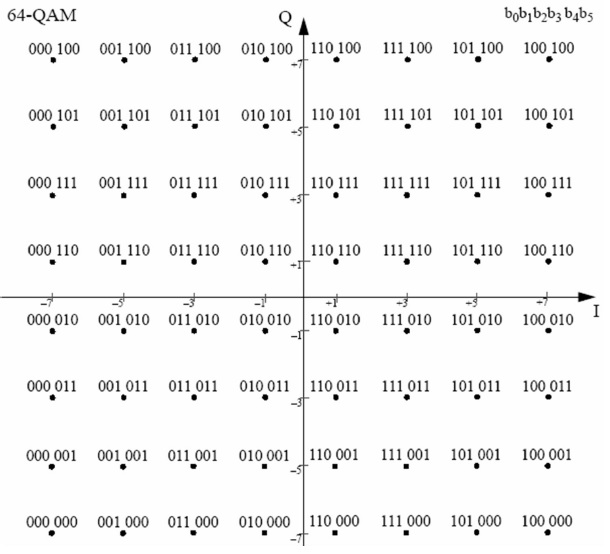
\includegraphics[width=9cm]{figure1.jpg}
\caption{Constellation diagram for 64-QAM}
\end{figure}

\subsection{Inter-Symbol Interference}
After passing through the communication channel the signal is decoded by a demodulator. The function of the demodulator is to classify each sample as a symbol. 
The performance of the fiber optic communication channels is often limited by a phenomenon known as dispersion, which causes optical pulses to broaden as they propagate through the fiber, thus giving rise to inter-symbol interference (ISI). 
Migration towards greater speed and longer links in fiber optic systems augment problems with dispersion in optical fibers, and dispersion compensation is consequently an increasingly important issue. Due to the ISI, the demodulator may misidentify that sample as other symbol, resulting in a symbol error.

\section{Challenge Addressed} %%%%%%%%%%%%%%%%%%%%%%

Taking in consideration the ISI problem, research teams are now looking for a viable answer to the demands of proper symbol identification by the demodulator at the end of the fiber optic communication channel. Today, with the progression made on the field of Machine Learning, the solution may be closer than never before.

Our goal for this project was to apply machine learning methods to compensate the inter-symbol interference and correctly decode the symbols that have been transmitted through an optical communication channel and collected from the noisy samples obtained by the receiver. The available data distribution through the optical channel is visible on the constellation diagram in Figure 2.

\begin{figure}[H]
\centering
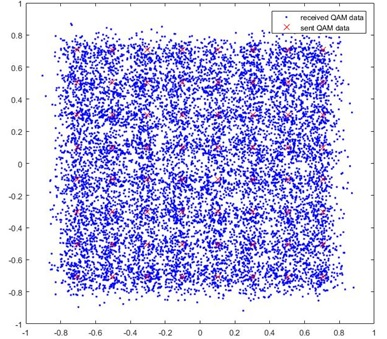
\includegraphics[width=9cm]{figure2.jpg}
\caption{Constellation diagram for rectangular 64-QAM transmitted (red crosses) and received (blue dots) symbols, using 10\% of the collected data}
\end{figure}

As proposed by professor Pétia Georgieva, we focused on the approach of considering the channel equalization as a classification problem with 64 classes and building a reliable classifier. The chosen classifier was the more promising candidate for this context, the Artificial Neural Network.

\section{Research} %%%%%%%%%%%%%%%%%%%%%%

The first steps for the concretion of a reliable solution began with taking in consideration the most significant issues inherent to the nature of the problem. These were how would an ANN consider 64 classes in a feasible and efficient manner, what would the best input parameters be and how can the best values for the ANN's hyperparameters be found in the minimum amount of time. After taking in consideration some proposals for these questions, the solution's structure resulted as presented bellow, but before we make available a small contextualization about Neural Networks and how they work.
All the development was made using Matlab, with the help of the matlab functions fmincg() (by Carl Edward Rasmussen) and nnCostFunction(), randInitializeWeights() and sigmoidGradient() (by Pétia Georgieva).

\subsection{Neural Networks}
Artificial Neural Networks are computing systems inspired by the biological neural networks of animal brains. The neural network is not an algorithm, but rather a framework for different machine learning algorithms to process complex data inputs. These systems "learn" to perform tasks by analysing examples, without being programmed with any specific rules.
The network consists of several levels of neurons that work together to learn something from the data that they are exposed to. This learning process envolves a standard of wrong and right that each neuron follows as is given by a cost function. The formula used in this study for the cost function is present next.

\begin{figure}[H]
\centering
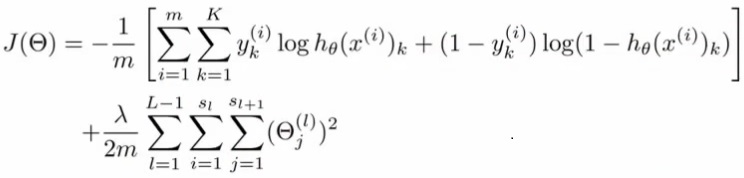
\includegraphics[width=9cm]{costfunctionformula.jpg}
\caption{Cost function formula for the ANNs}
\end{figure}

The connections between artificial neurons are called 'edges'. Artificial neurons and edges typically have a weight (or theta value) that adjusts as learning proceeds. The weight increases or decreases the strength of the signal at a connection, meaning that different neurons will have different influences on the decisions of the whole network. The training of a Neural Network starts with a random initialization of these theta values. The final step (reffered in chapter V) considers the validation and training data and passes it to the ANNs (running the algorithm once again) now with the theta values resultant from the previous steps.

\subsection{Architecture}
The first answer turned out to be rather intuitive and lowered the complexity of the ANN in a considerably great amount. The idea consisted in dividing the problem in two Neural Networks.
As it is known, the signal sent through the optical channel is represented with a complex number (with a real value and an imaginary value) - this allows for the classifier to deal with the real data separated from the imaginary data. With this in mind, if two ANN where able to correctly classify the values of their nature (one responsible for the real values, the other for the imaginary ones), then adding the result of each classification would also return the correct classification of the original complex number.
The visualization of these two Neural Networks is present in Figure 4 (details about the input parameters are explained next).

\subsection{Data Nature}
Defining what are the best features for the ANNs is a more difficult task, since no answer is really correct or incorrect - only more or less appropriate and more or less effective for the problem at hands. 
With little documentation available regarding this, we decided to test the idea given by the Institute of Telecommunications of the University of Aveiro that consisted in taking in consideration that the data consisted in a stream of symbols where the current symbol is somehow related with the previous ones. So, to look for this relation, we fed the Neural Networks not only with the current symbol, but also with a certain amount of previous values. In Figure 4, the reader can analyse the features given to the ANNs.
This not only had the purpose of searching for good way of predicting the symbols' classes, but also to find out if the symbols of the stream close to the current one had any effect on its class. 

\begin{figure*}[h]
\centering
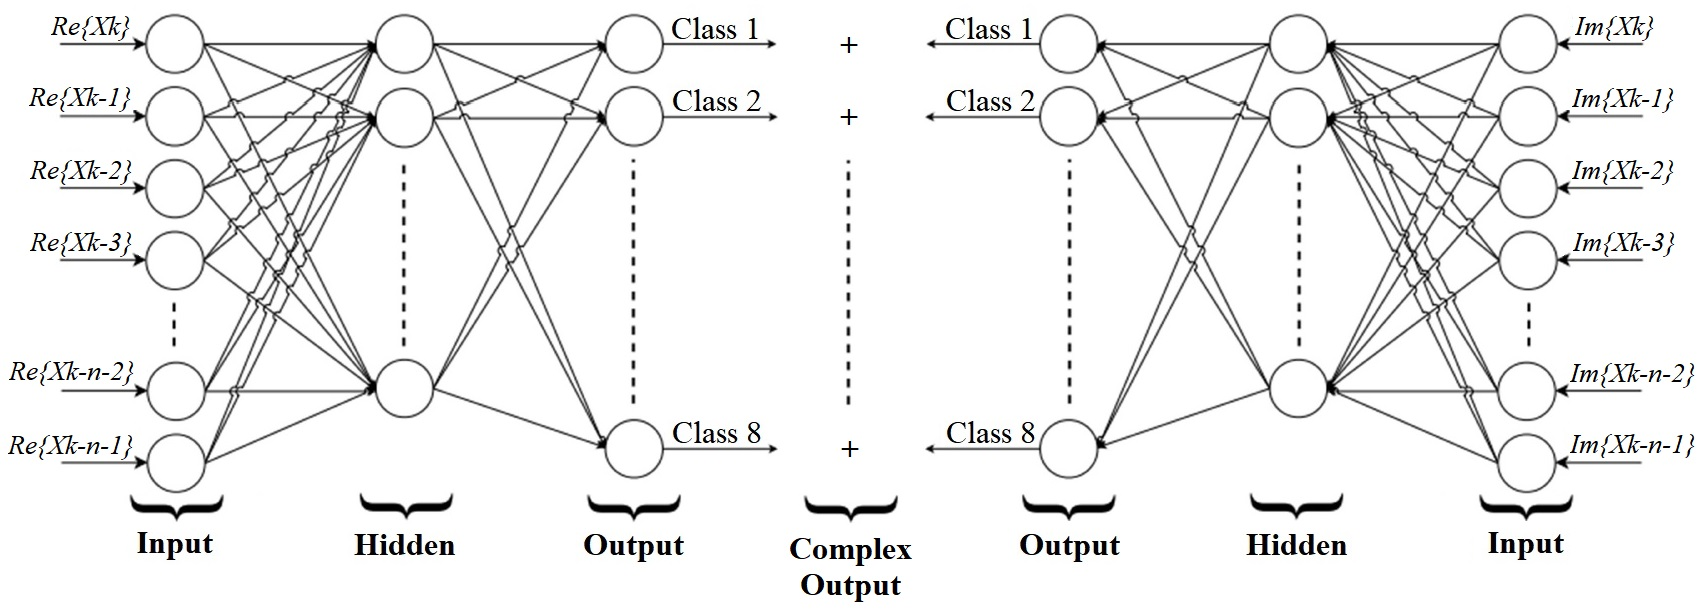
\includegraphics[width=\textwidth, height=6.8cm]{figure4.jpg}
\caption{Visual representation of the ANNs}
\end{figure*}

The dataset available for this study consisted in over 170 000 samples, meaning that a balacing between data processing and time available for research had to be discussed. It was here that the dataset was divided into 3 groups: the first and largest for training the ANNs, holding 60\% of the samples; the validation group, with 20\%; and the testing group, with the remaining 20\%, only used in the analysis of the system's final solution.

\subsection{Hyperparameter Weights}
After implementing the base architecture of the classifier and dividing the dataset by groups, our attention shifted towards the hyperparameters involved. These are: the number of features of each ANN, the learning rate (Lambda), the number of hidden layer neurons and the number of Epochs. Given that the data available was of a considerable large size and the time available to work with them was short, we had to compromise the variations of values of each hyperparameter. Table 1 shows the combinations of values we chose for this study - these were decided giving priority to the weight of each one and the importance of finding out their behaviour on the learning process. It is important to reffer that the lambda values were chosen after a few preliminary tests on how did the ANNs respond to the variation of the learning rate.

\FloatBarrier
\begin{table}[h]
\resizebox{\columnwidth}{!}{%
\begin{tabular}{|l|l|l|l|}
\hline
\textbf{\# Features} & \textbf{Lambda} & \textbf{\# ANN Neurons} & \textbf{\#  Epochs} \\ \hline
1 & 0 & 10 & 100 \\ \hline
2 & 0 & 10 & 100 \\ \hline
3 & 0 & 10 & 100 \\ \hline
4 & 0 & 10 & 100 \\ \hline
1 & 0.3 & 10 & 100 \\ \hline
2 & 0.3 & 10 & 100 \\ \hline
3 & 0.3 & 10 & 100 \\ \hline
4 & 0.3 & 10 & 100 \\ \hline 
\end{tabular}%
}
\caption{Combinations of hyperparameters tested}
\end{table}
\FloatBarrier

\section{Analysis} %%%%%%%%%%%%%%%%%%%%%%

After training the ANNs for each combination of hyperparameter values and calculating their accuracies, some conclusions were visible. 
The most important conclusion is related to the basis of our study - the features selection. Analysing Figures 5 and 6, the almost constant values of the accuracies make it clear that trying to relate the current symbol received with previous ones has little to no effect on the class that it belongs to. The predictions fail approximately 2 times out of 10, whether the ANNs take in consideration 3 previous symbols or none. 

Another observation made was that the best combinations for predicting the real values are not the same for the imaginary values. However, we believe that this is not relevant for our case study and we only use the best combinations found to consider the best cenario for each ANN and find out the best possible outcome (see chapter V).

The final observation is one worth taking a closer look, even though it comes quite naturally. Analysing all tests made, even though the singular accuracies of each ANN were fairly high (~89\%), when combining them to calculate the accuracy of the complex number prediction this value would lower to the already mentioned ~80\%. This is due to the phenomenon of mismatch between predictions - easily understanted in Figure 7. The basic understanding here is that even a correct prediction of one ANN does not guarantee that the other will also correctly predict the respective value, causing additional error to the final predictions.

\section{Best Solution} %%%%%%%%%%%%%%%%%%%%%%

\begin{table}[]
\resizebox{\columnwidth}{!}{%
\begin{tabular}{|l|l|l|l|l|}
\hline
\textbf{Real Accuracy} & \textbf{Imaginary Accuracy} & \textbf{Total Accuracy} \\ \hline
89.1958 & 88.2049 & 78.7817 \\ \hline
\end{tabular}%
}
\caption{Performance of the system's final version in \%}
\end{table}

Once finished with the Analysis phase, the study proceeded to improving the capabilities of the system using the best found values for the ANNs. This process envolved using the best Theta values from the previous steps and running the algorithm one final time giving as input the training and validation data. Finally, we use the testing data (stored since the beggining of the study and never touched) to validate the final stage of the system, calculating the predictions based on the new and improved theta values and comparing them to the corresponding labels.
The performance of the system is shown in Table 2, where we can see the accuracy of the final solution.

\begin{figure}[h]
\centering
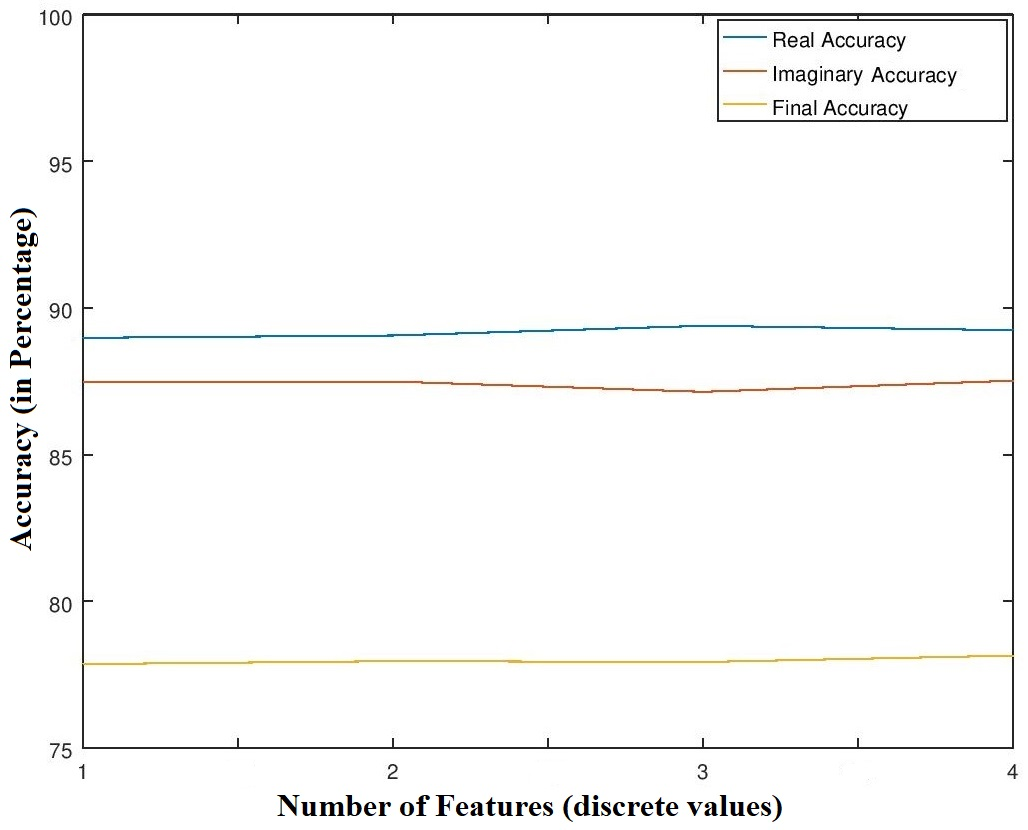
\includegraphics[width=9cm, height=8cm]{lambda0.jpg}
\caption{Accuracies for lambda=0.0, varying the number of previous symbols fed to the ANNs (from 0 to 3)}
\end{figure}

\begin{figure}[h]
\centering
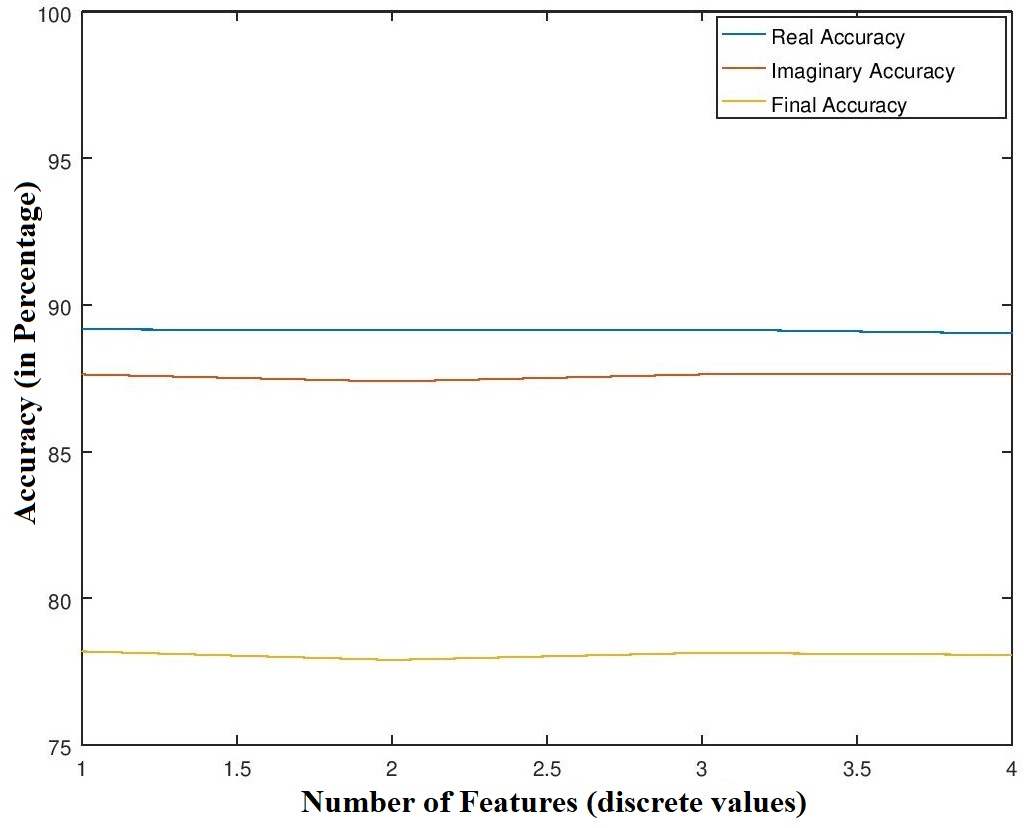
\includegraphics[width=9cm, height=8cm]{lambda03.jpg}
\caption{Accuracies for lambda=0.3, varying the number of previous symbols fed to the ANNs (from 0 to 3)}
\end{figure}

\section{Conclusions and Future Work} %%%%%%%%%%%%%%%%%%%%%%

\begin{figure}[h]
\centering
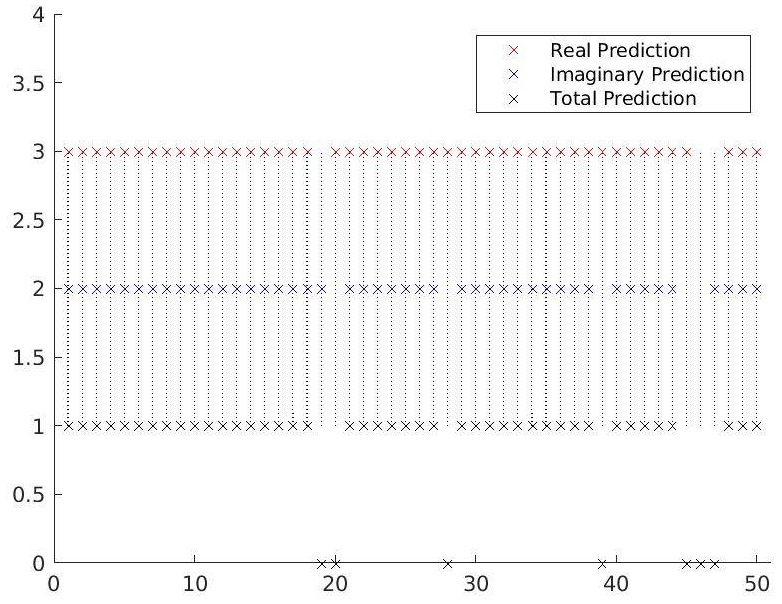
\includegraphics[width=9cm]{mismatch.jpg}
\caption{Visualization of the mismatch between predictions of the Real and the Imaginary ANNs (points on Xaxis show mismatch occurrences)}
\end{figure}

The overall results of our research were bellow the expectations, since any classifier with an accuracy bellow 99\% is not welcomed in the world of optical communications. We gather that the assumption that other symbols on the signal stream could influence the class of the symbol being classified might be partially incorrect, or at least their weights may be of little effect. This means that it is quite possible that another source of information is influencing more the current symbol and that it should be considered by the ANNs for a better predicition.

The next step for this hunt could be to adopt a new strategy for the ANNs' features, such as considering a class as isolated and calculating the distances between the received signal (with ISI) and all the real classes and compare this study's results with the new ones. We believe that the distances will tell us with a more accurate predicition to which class does the signal belong to, since the received signals seem to follow a gaussian distribuition (see Figure 2) and naturally fall closer to their class. The collected knowledge made it clear that Neural Networks can be one future solution for this big challenge and are today one step closer to finding it.



\end{document}